\newchapter{intro}{Introduction}

This is the introductory text.

%\newsection{partPhys}{Particle Physics}

%\newsection{accelIntro}{Particle Colliders}

\newsection{linColliderIntro}{Motivation for Future Linear Colliders}

what colliders are/what they are for

why want a e+ e- collider

why linear better for e+ e-

two proposals - ILC and CLIC. ILC up to 1 TeV. CLIC up to 3 TeV. ILC more mature/could be built now. CLIC more challenging.

\newsection{clicIntro}{CLIC}

basics of main beam, length etc.

accelerating gradient - why need it to be high, why 12 GHz chosen

drive beam - why (efficiency/cost vs. 12 GHz klystrons), combination process, PETS


%\newsection{fontIntro}{FONT}

\newsection{clicPFF}{Phase Feedforward for CLIC}

phase jitter vs. luminosity

expected phase jitter plot

source of phase jitter

proposed layout of system to remove it - turnarounds before extraction. beat timing of beam etc.

required specifications - hardware power, bandwidth, latency etc.

\newsection{ctfIntro}{CTF3}

\subsection{Goals of CTF3}
\label{ss:ctfGoals}

prove main CLIC concepts, drive beam generation, accelerating cavities, etc.

PFF prototype

\subsection{Layout of CTF3}
\label{ss:ctfLayout}

basic parameters: 3GHz/1.5GHz beam, up to factor 8, initial 3-4A, final up to 26A(?)

sections: linac, CT, DL, TL1, CR, TL2, CLEX (TBL/TBTS), CALIFES

\begin{figure}
  \centering
  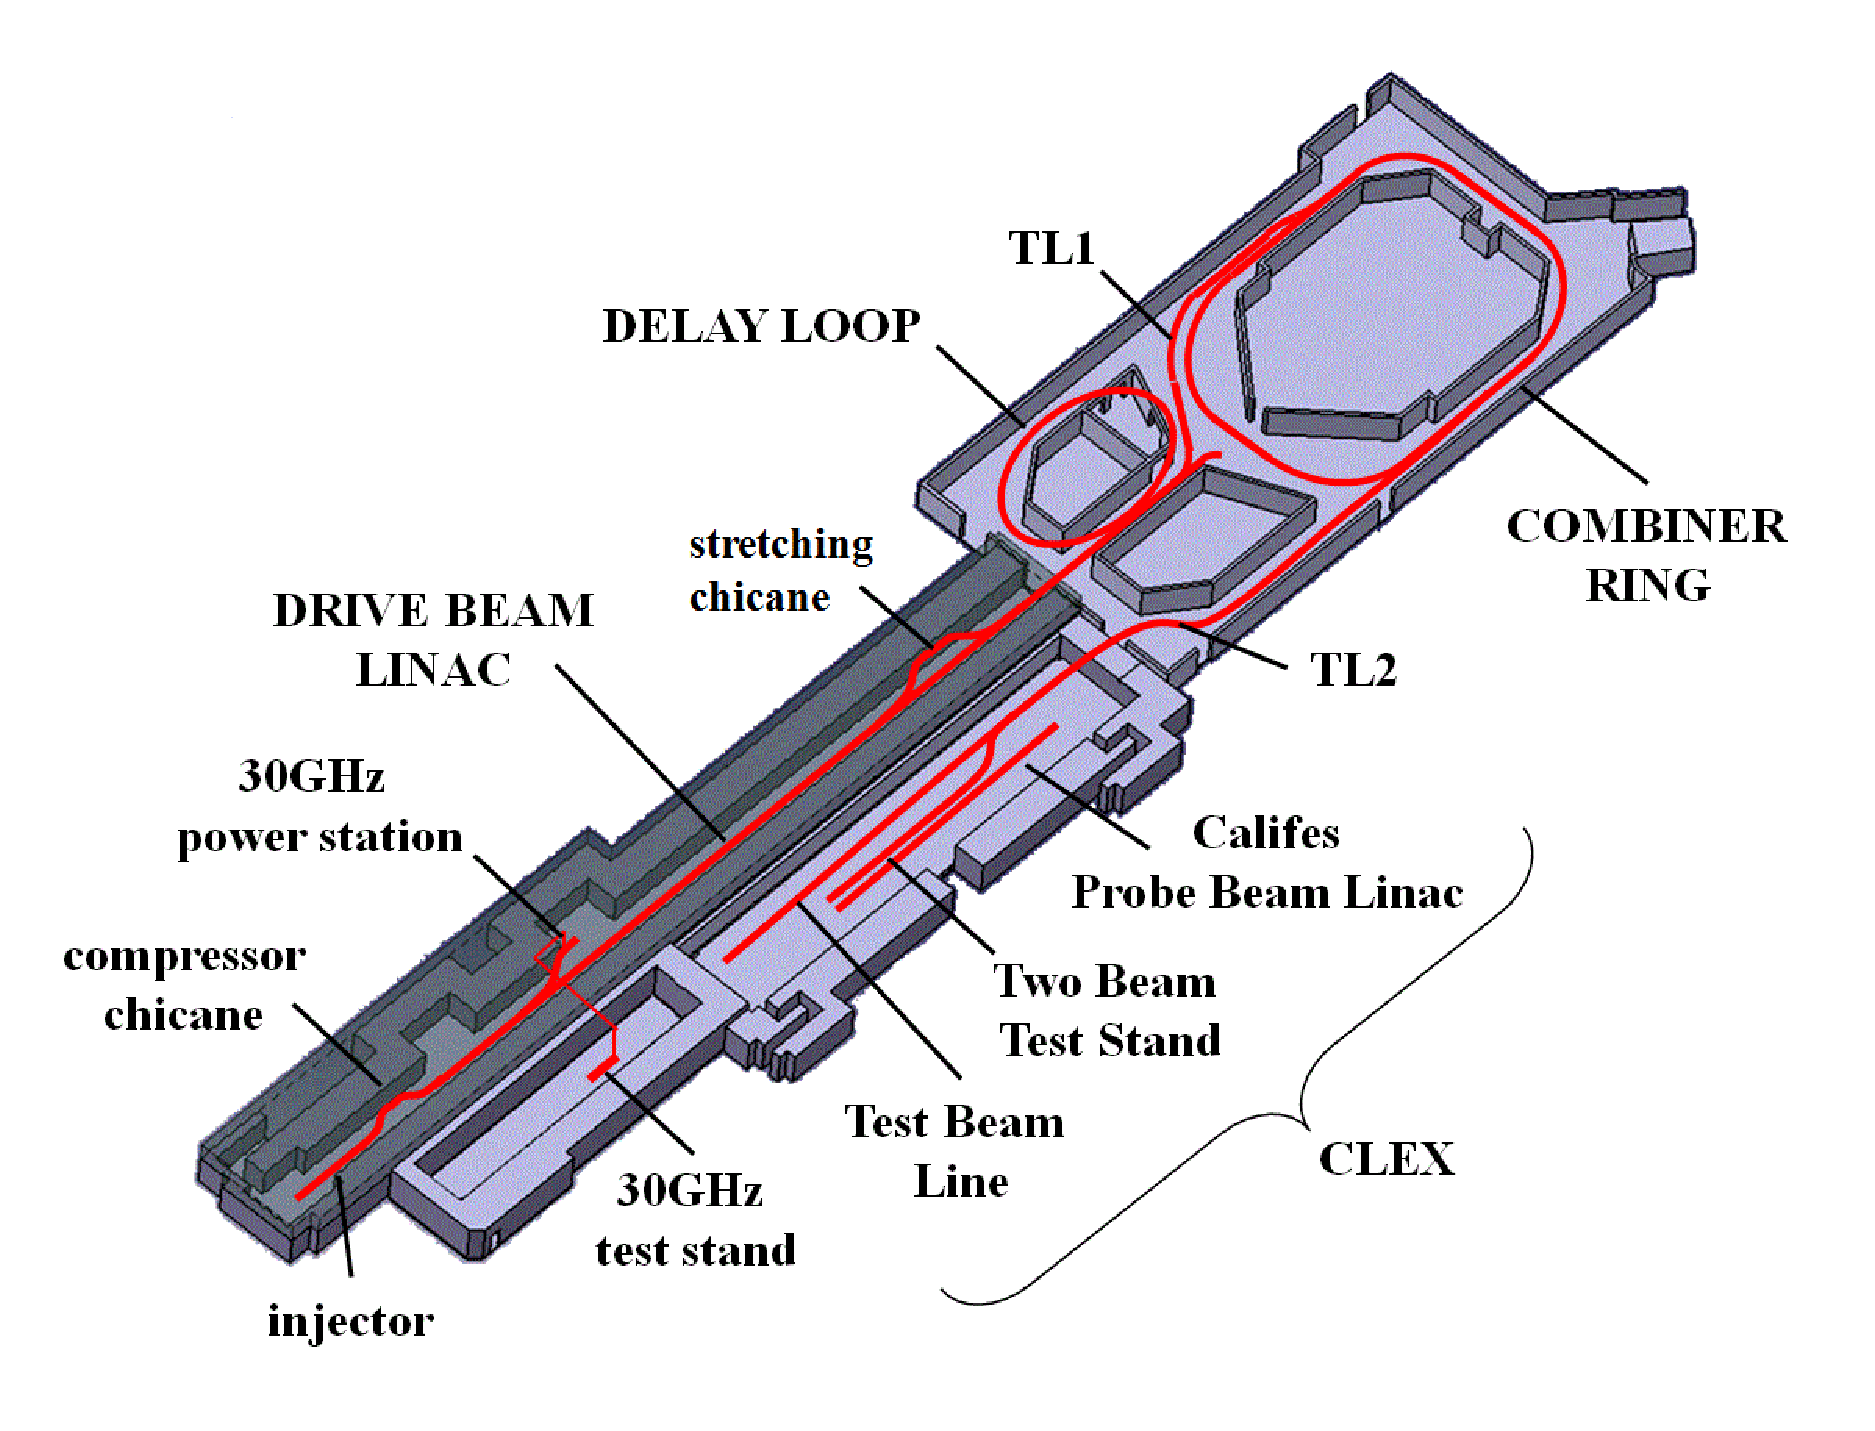
\includegraphics[width=0.45\textwidth]{Figures/ctfLayout}
  \caption{CTF3 schematic.}
  \label{f:ctfLayout}
\end{figure}

\newsection{pffCTFIntro}{Design of the PFF Prototype at CTF3}

\subsection{Schematic Overview of PFF System}
\label{ss:ctfPFFLayout}

location of hardware - CT phase mons, TL2 kickers, TBL phase mon.

diagram of hardware locations

correction range/general targets

\subsection{Hardware}
\label{ss:ctfPFFHardware}

who built the hardware

references to chapters/sections where they are discussed

\subsection{Latency}
\label{ss:availLatency}

beam TOF CT->TL2 chicane

\subsection{Differences Between PFF at CTF and CLIC}
\label{ss:ctfVsCLIC}

The goal of the prototype is to prove the general PFF concept and the feasibility of using it to achieve \(0.2^\circ\) drive beam phase stability. It is neither necessary nor possible for the proposed CLIC and CTF3 systems to be identical, and there are a number of differences between the two that are summarised here. 

The most obvious difference is the design of the correction chicane -- with a four bend C--shaped chicane with four PFF kickers installed proposed for CLIC, compared to the four bend dog leg chicane at CTF3 with two PFF kickers installed for the correction. The freedom to design a purpose built chicane with additional kickers in the CLIC design somewhat simplifies the challenges of obtaining a suitable layout for the prototype chicane at CTF3 using pre-existing hardware (Chapter~\ref{c:tl2Optics}).

Another key difference is that at CTF3 the PFF prototype is operated on uncombined beam, bypassing the delay loop and completing only half a turn in the combiner ring. At CLIC the complete PFF system (including the PFF input) is placed after the drive beam recombination, and therefore would operate on combined beam. At CTF3 as the PFF input is placed prior to the delay loop any attempt to operate the PFF prototype with combined beam would be complicated by having to use the measured uncombined beam pulse to correct the combined pulse following the combiner ring. Nevertheless, operation of the prototype with combined beam could be possible and may be attempted in future tests.

The main effect of using the uncombined pulse at CTF3 rather than the combined pulse as forseen for CLIC is that the beam pulse lengths are different. At CLIC \(0.2^\circ\) phase stability is needed across the [TODO:howlong] combined beam pulse. At CTF3 the uncombined pulse is much longer, up to 1.2~\(\mathrm{\mu s}\). It is therefore not necessary to demonstrate \(0.2^\circ\) phase stability across the full CTF3 pulse length to fulfill the CLIC requirements.

In fact, it is in any case impossible to demonstrate \(0.2^\circ\) phase stability across the full CTF3 pulse length with the PFF prototype due to the large phase sag that is present along the beam pulse. The RF pulse compression system at CTF3 [REF] results in an approximately parabolic variation of roughly \(40^\circ\) along the pulse. This would not be present at CLIC. The phase sag is much larger than the correction range of the PFF prototype, which is designed to remove smaller, fast offsets. The PFF correction is therefore focused on the flatter, central part of the pulse around the peak of the phase sag, where the phase variations across the pulse length relevant for CLIC are within the correction range.


\newsection{phaseJitDefs}{Definitions of Different Phase Statistics}

Throughout the thesis several terms will be use to describe different ways of measuring the phase, as well as other parameters. These terms are briefly summarised here for reference. All quoted phase values throughout the thesis are in degrees at 12~GHz.

CTF3 provides an uncombined beam pulse length of up to 1.2~\(\mathrm{\mu s}\). It is useful to compare results both along the pulse and for the mean of the pulse. To calculate ``mean'' statistics, the average of each beam pulse is taken. Usually this is not taken across the full pulse length, but rather across a a region of several hundred nanoseconds near the mid-portion of the pulse where the beam is most stable and the phase sag is flattest. Mean statistics are usually plotted against time in units of the pulse number, with CTF3 operating at a repetition rate of 0.8~Hz, or one beam pulse every 1.25~s. The mean phase jitter represents the standard deviation of these mean values across the duration of a dataset.

Any statistic instead described as being ``along the pulse'' represents the measured values point by point along the beam pulse, typically sampled at a rate of a few hundred MHz. The time axes for plots of statistics along the pulse are either in units of nanoseconds, or simply the point number along the pulse (sample number). The phase jitter along the pulse represents the standard deviation of the measured phases at each individual sample point taken across the duration of a dataset.

Many of the discussions in the thesis also quote correlation coefficients, which in all cases are Pearson product-moment correlation coefficients [REF].

\newsection{thesisOverview}{Thesis Overview}

This thesis documents the design, commissioning, operation and results of the PFF prototype at CTF3. In Chapter~\ref{c:tl2Optics} the design of the TL2 chicane and the modifications to it that were necessary to achieve the desired phase shifting behaviour are described in more detail. 

The performance of the PFF correction depends on the ability to precisely measure the beam phase, and so Chapter~\ref{c:phaseMons} presents the extensive work that has been completed to understand and maximise the precision of the new purpose built phase monitors that were installed at CTF3 for the PFF system. 

As well as excellent precision in the measured phase, it is crucial to have high correlation between the phase at the end of the linac (the PFF input) and the phase at the correction location (TL2). With no correlation between the phases at these two points no improvement in phase jitter would be possible with the PFF system. Chapter~\ref{c:phasePropagation} describes the process of understanding and improving this correlation.

Chapter~\ref{c:commissioning} focuses on the setup of the remaining PFF hardware components and the commissioning of the complete PFF system. This includes the implementation of the PFF correction on the feedforward controller (the FONT5a board), the design and performance of the kicker amplifiers, as well as verifying the correction timing and correction range.

Chapter~\ref{c:feedforward} then presents the best results that have been achieved with the PFF prototype to date following all the optimisations described in the rest of the thesis. An analysis of the current limitations of the system and possible future improvements to the PFF setup are also discussed. Finally, the conclusions from each chapter and suggestions for future work are summarised in Chapter~\ref{c:conclusion}.

